\chapter{\label{chap:chap4} Ambiente de simulação e estudos de caso}
% Sérgio: Este capítulo poderia se chamar "Ambiente de simulação e estudos de caso"

\section{Ambiente de simulação}
% Seção: "Ambiente de simulação" - descrever como tu montou tuas simulações, e como foi organizado o ambiente, etc..
Em um primeiro momento a névoa foi construída de forma simulada utilizando a ferramenta Common Open Research Emulator (CORE)\cite{coregui}.
Para os primeiros experimentos a ferramente obteve resultados satisfatórios, porém quando foi necessário escalarmos a solução ela se mostrou ineficiente.
A ineficiência estava na criação dos nodos e na execução dos protocolos CoAP e Resource Mapping, uma vez que eles deveriam ser executados em todos os hosts da rede e não havia 
meios de automatizar este processo.

Esta automatização foi implantada utilizando a SDK de gerenciamento de containers Docker para Python, desta forma, foi possível criarmos névoas com tamanhos arbitrários
e, portanto, a ascalabilidade da solução pode ser amplamente testada\cite{dockersdk:2018}.

Cabe ressaltar que containers Docker\cite{docker:2018} consomem recursos da maquina hospedeira, tais como memória, processamento, disco rígido.
Portanto, a criacao de containers da névoa fica atrelado a quantidade de recursos que esse host pode proporcionar.

Cada container executa uma distrbuição Linux chamada Alpine, de aproximadamente 5Mb, que possui apenas as funcioalidades básicas de um sistema operacional\cite{linuxalpine:2018}.
O fato da distribuição ser Open Source faz com que existam customizações da mesma, e neste projeto foi utilizado a customização que inclui a versão 2.7 da linguagem Python.
Tal customização faz-se necessária para a execução dos protocolos CoAP e Resource Mapping.


A Figura \ref{fig:fig13} não só expõe os elementos que fazem parte da arquitetura de cada container, mas também os detalha em nível de requisições entre sí.


\begin{figure}[H]
    \centering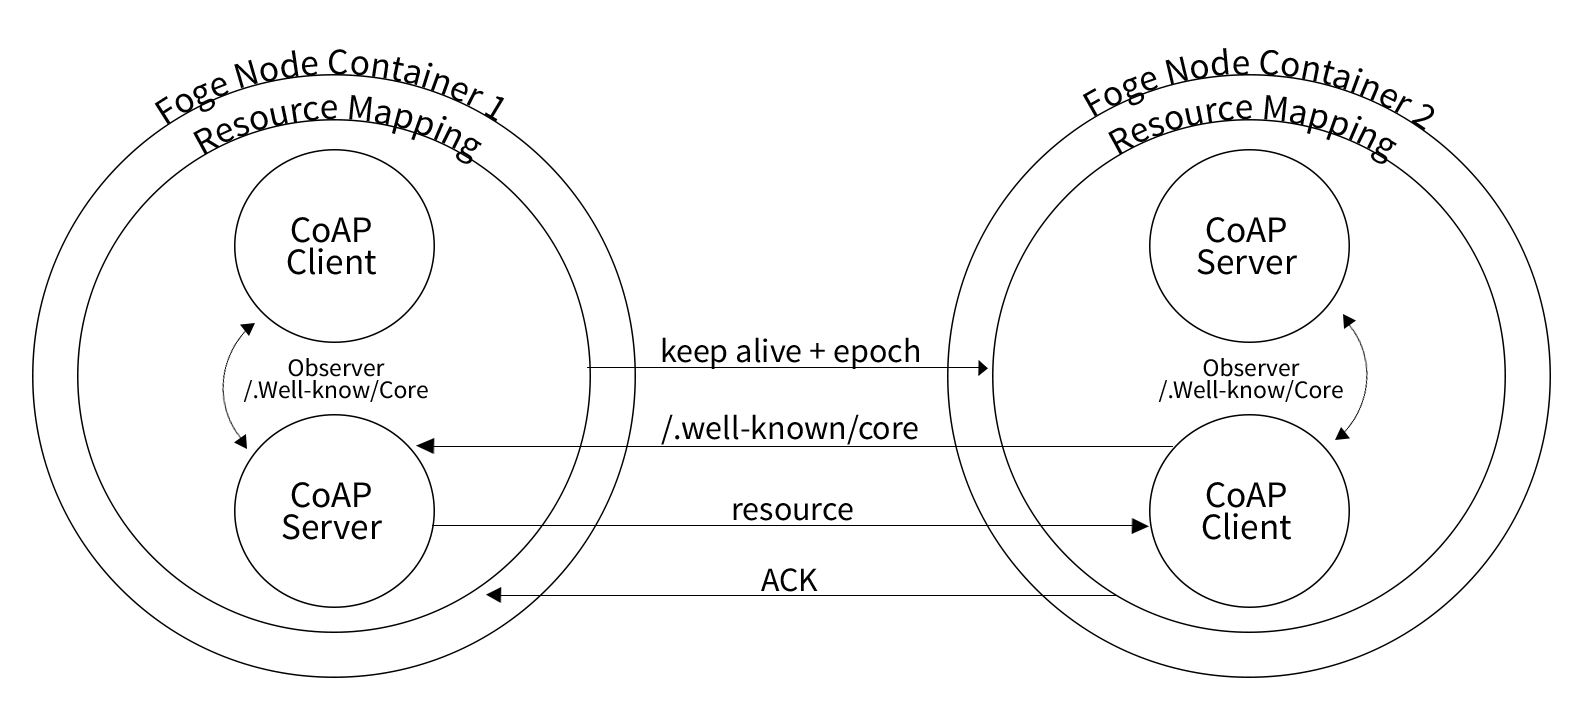
\includegraphics[width=.8\textwidth]{fig13.png}
    \caption%[This figure has a shorter caption now]%
    {\label{fig:fig13} Fog node container.}
\end{figure}


Além do protocolo de mapeamento em sí, este trabalho dispõe de uma API para o gerenciamento de recursos providos pelos CoAP servers.
Esta API possui métodos para listagem, remoção e criação de recursos e deve ser executada a partir do host que gerencia os container.
Assim, conseguimos proporcionar o dinamismo que a névoa necessita para a realização de testes no comportamento do protocolo de sincronização.



\section{Cenários de teste}
% Seção: "Cenários de teste"

% A validação deste trabalho consiste em realizar simulações que faça com que o protocolo execute suas funcionalidades de acordo com os resultados descritos na Seção anterior, sendo assim, 
% algumas situações devem ocorrer para que as validações sejam realizadas.
% Estas situações serão abordadas nos cenários de teste da Seção a seguir.


Utilizando como base a Figura \ref{fig:fig7}, e partindo do pressuposto que todos os nodos da névoa já estão com seus recursos sincronizados corretamente,
iremos exemplificar os cenários de testes elencados abaixo.

\begin{enumerate}
    \item Entrada de algum equipamento na rede e este anunciando seus recursos. 
    \item Atualização das listas globais quando algum equipamento deixar de responder as mensagens de keep alive.
    \item Atualização da lista de recursos quando algum edge device é adicionado ou removido de um nodo da névoa.
\end{enumerate}

\begin{figure}[H]
    \centering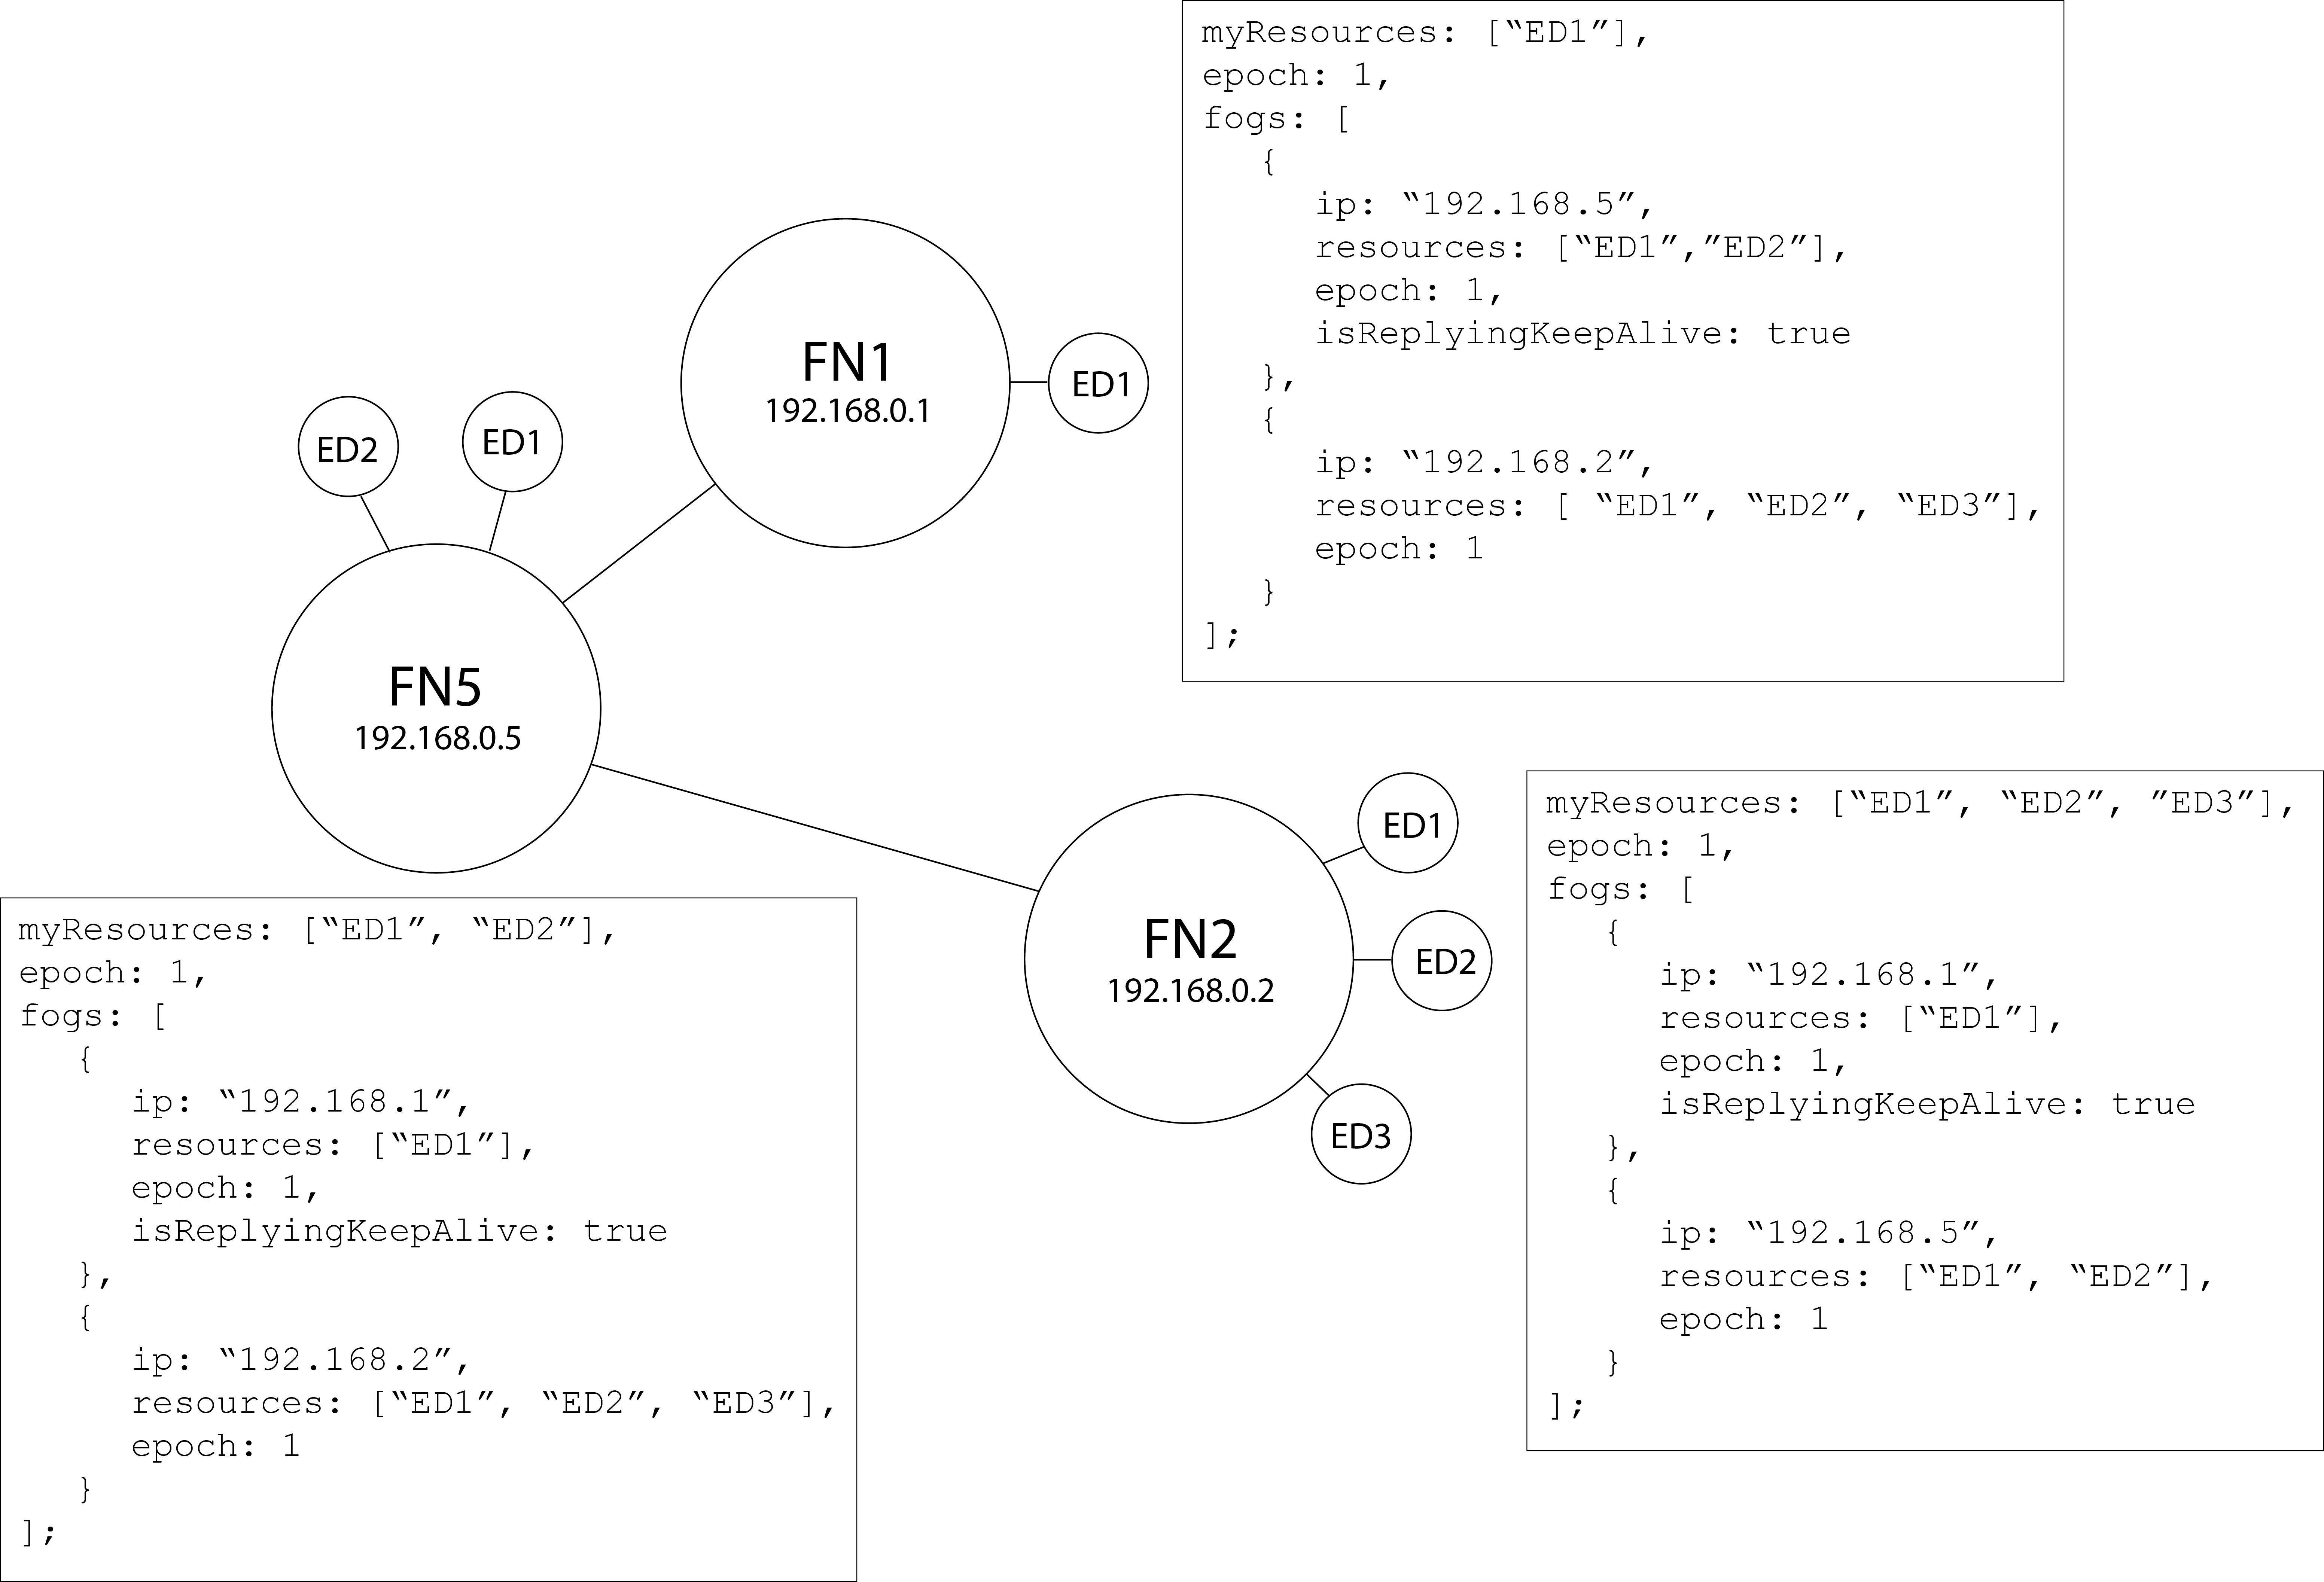
\includegraphics[width=.8\textwidth]{fig7.png}
    \caption%[This figure has a shorter caption now]%
    {\label{fig:fig7} Topologia base para cenário de teste.}
\end{figure}

O item 1 não será demonstrado agora, uma vez que as Subseções 3.2.2 e 3.2.3 já o fizeram, portanto, partiremos diretamente para o segundo item da listagem.

O segundo item trata-se de quando um nodo deixa de responder mensagens de keep alive, e a Figura \ref{fig:fig7} será utilizada para ilustrar este funcionamento.
Na Figura \ref{fig:fig8}, o nodo FN1 não respondeu, no tempo previamente estipulado, a mensagem de keep alive enviada pelo nodo FN2, 
portanto, o nodo destinatário foi marcado em FN2 como parcialmente inativo.


\begin{figure}[H]
    \centering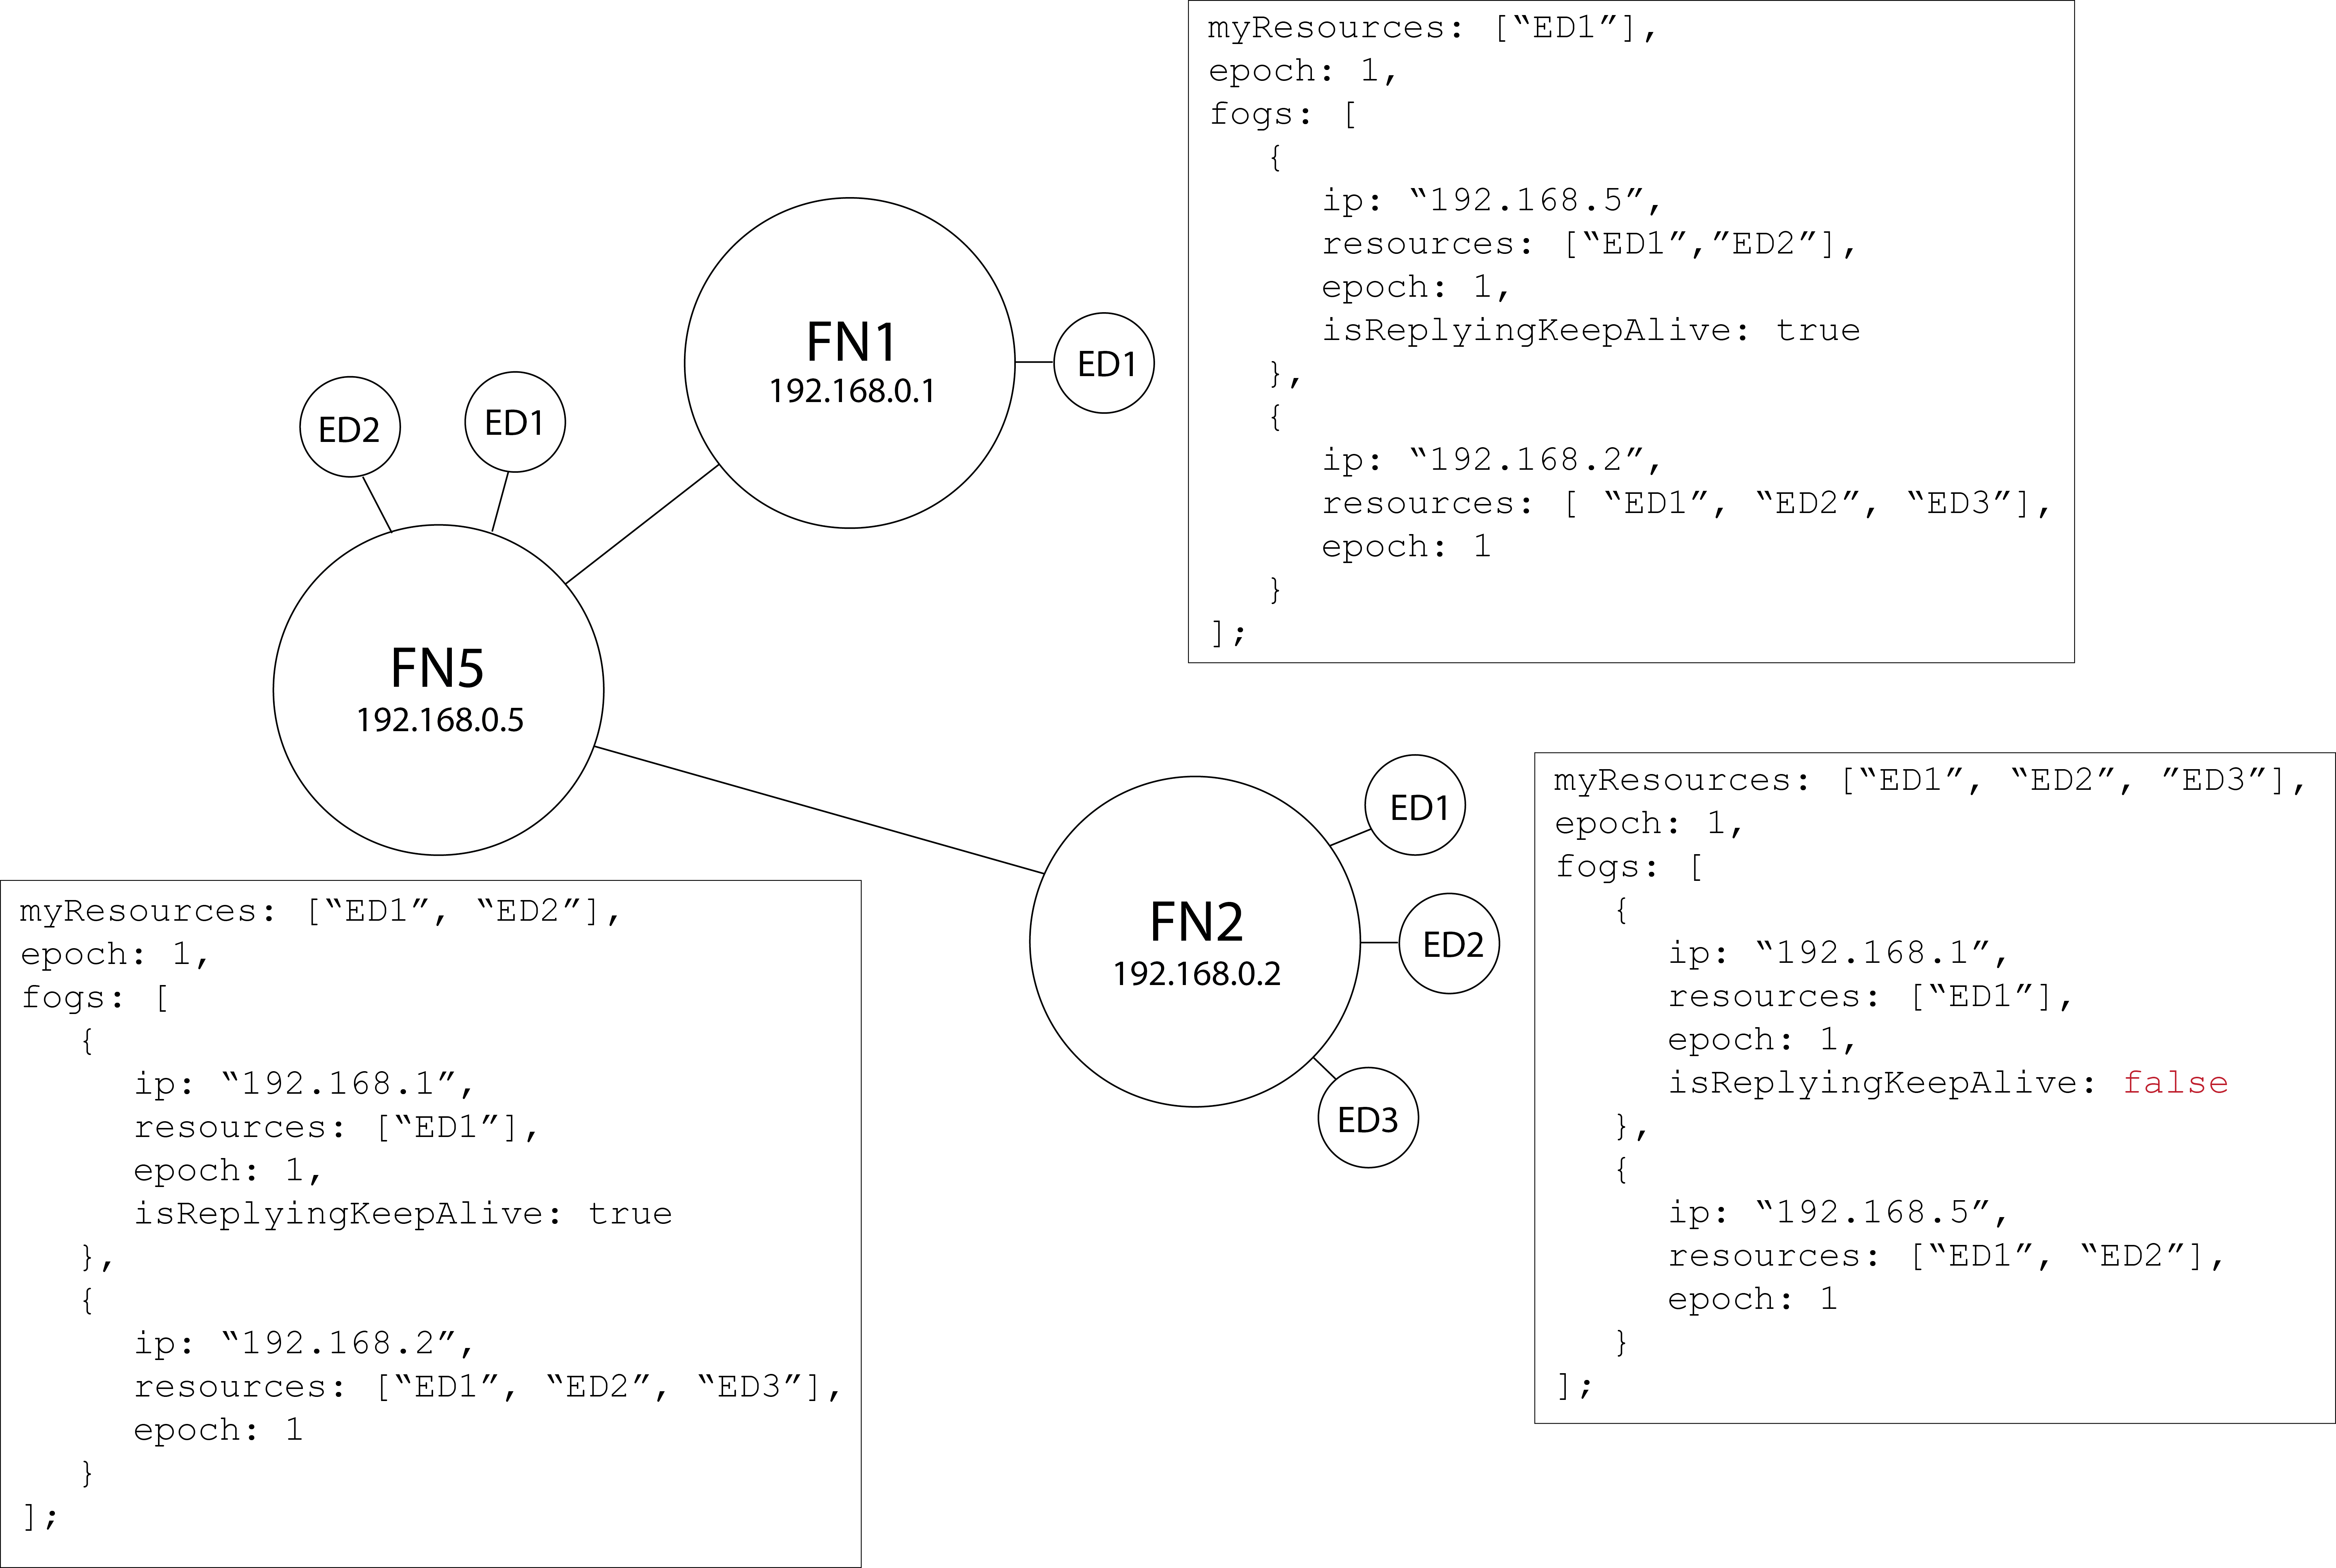
\includegraphics[width=.8\textwidth]{fig8.png}
    \caption%[This figure has a shorter caption now]%
    {\label{fig:fig8} Nodo marcado como parcialmente inativo.}
\end{figure}

Já a Figura \ref{fig:fig9} demonstra que o nodo FN1 não respondeu novamente à mensagem de keep alive enviada por FN2, por isso, foi removido de sua lista de recursos. 

\begin{figure}[h!]
    \centering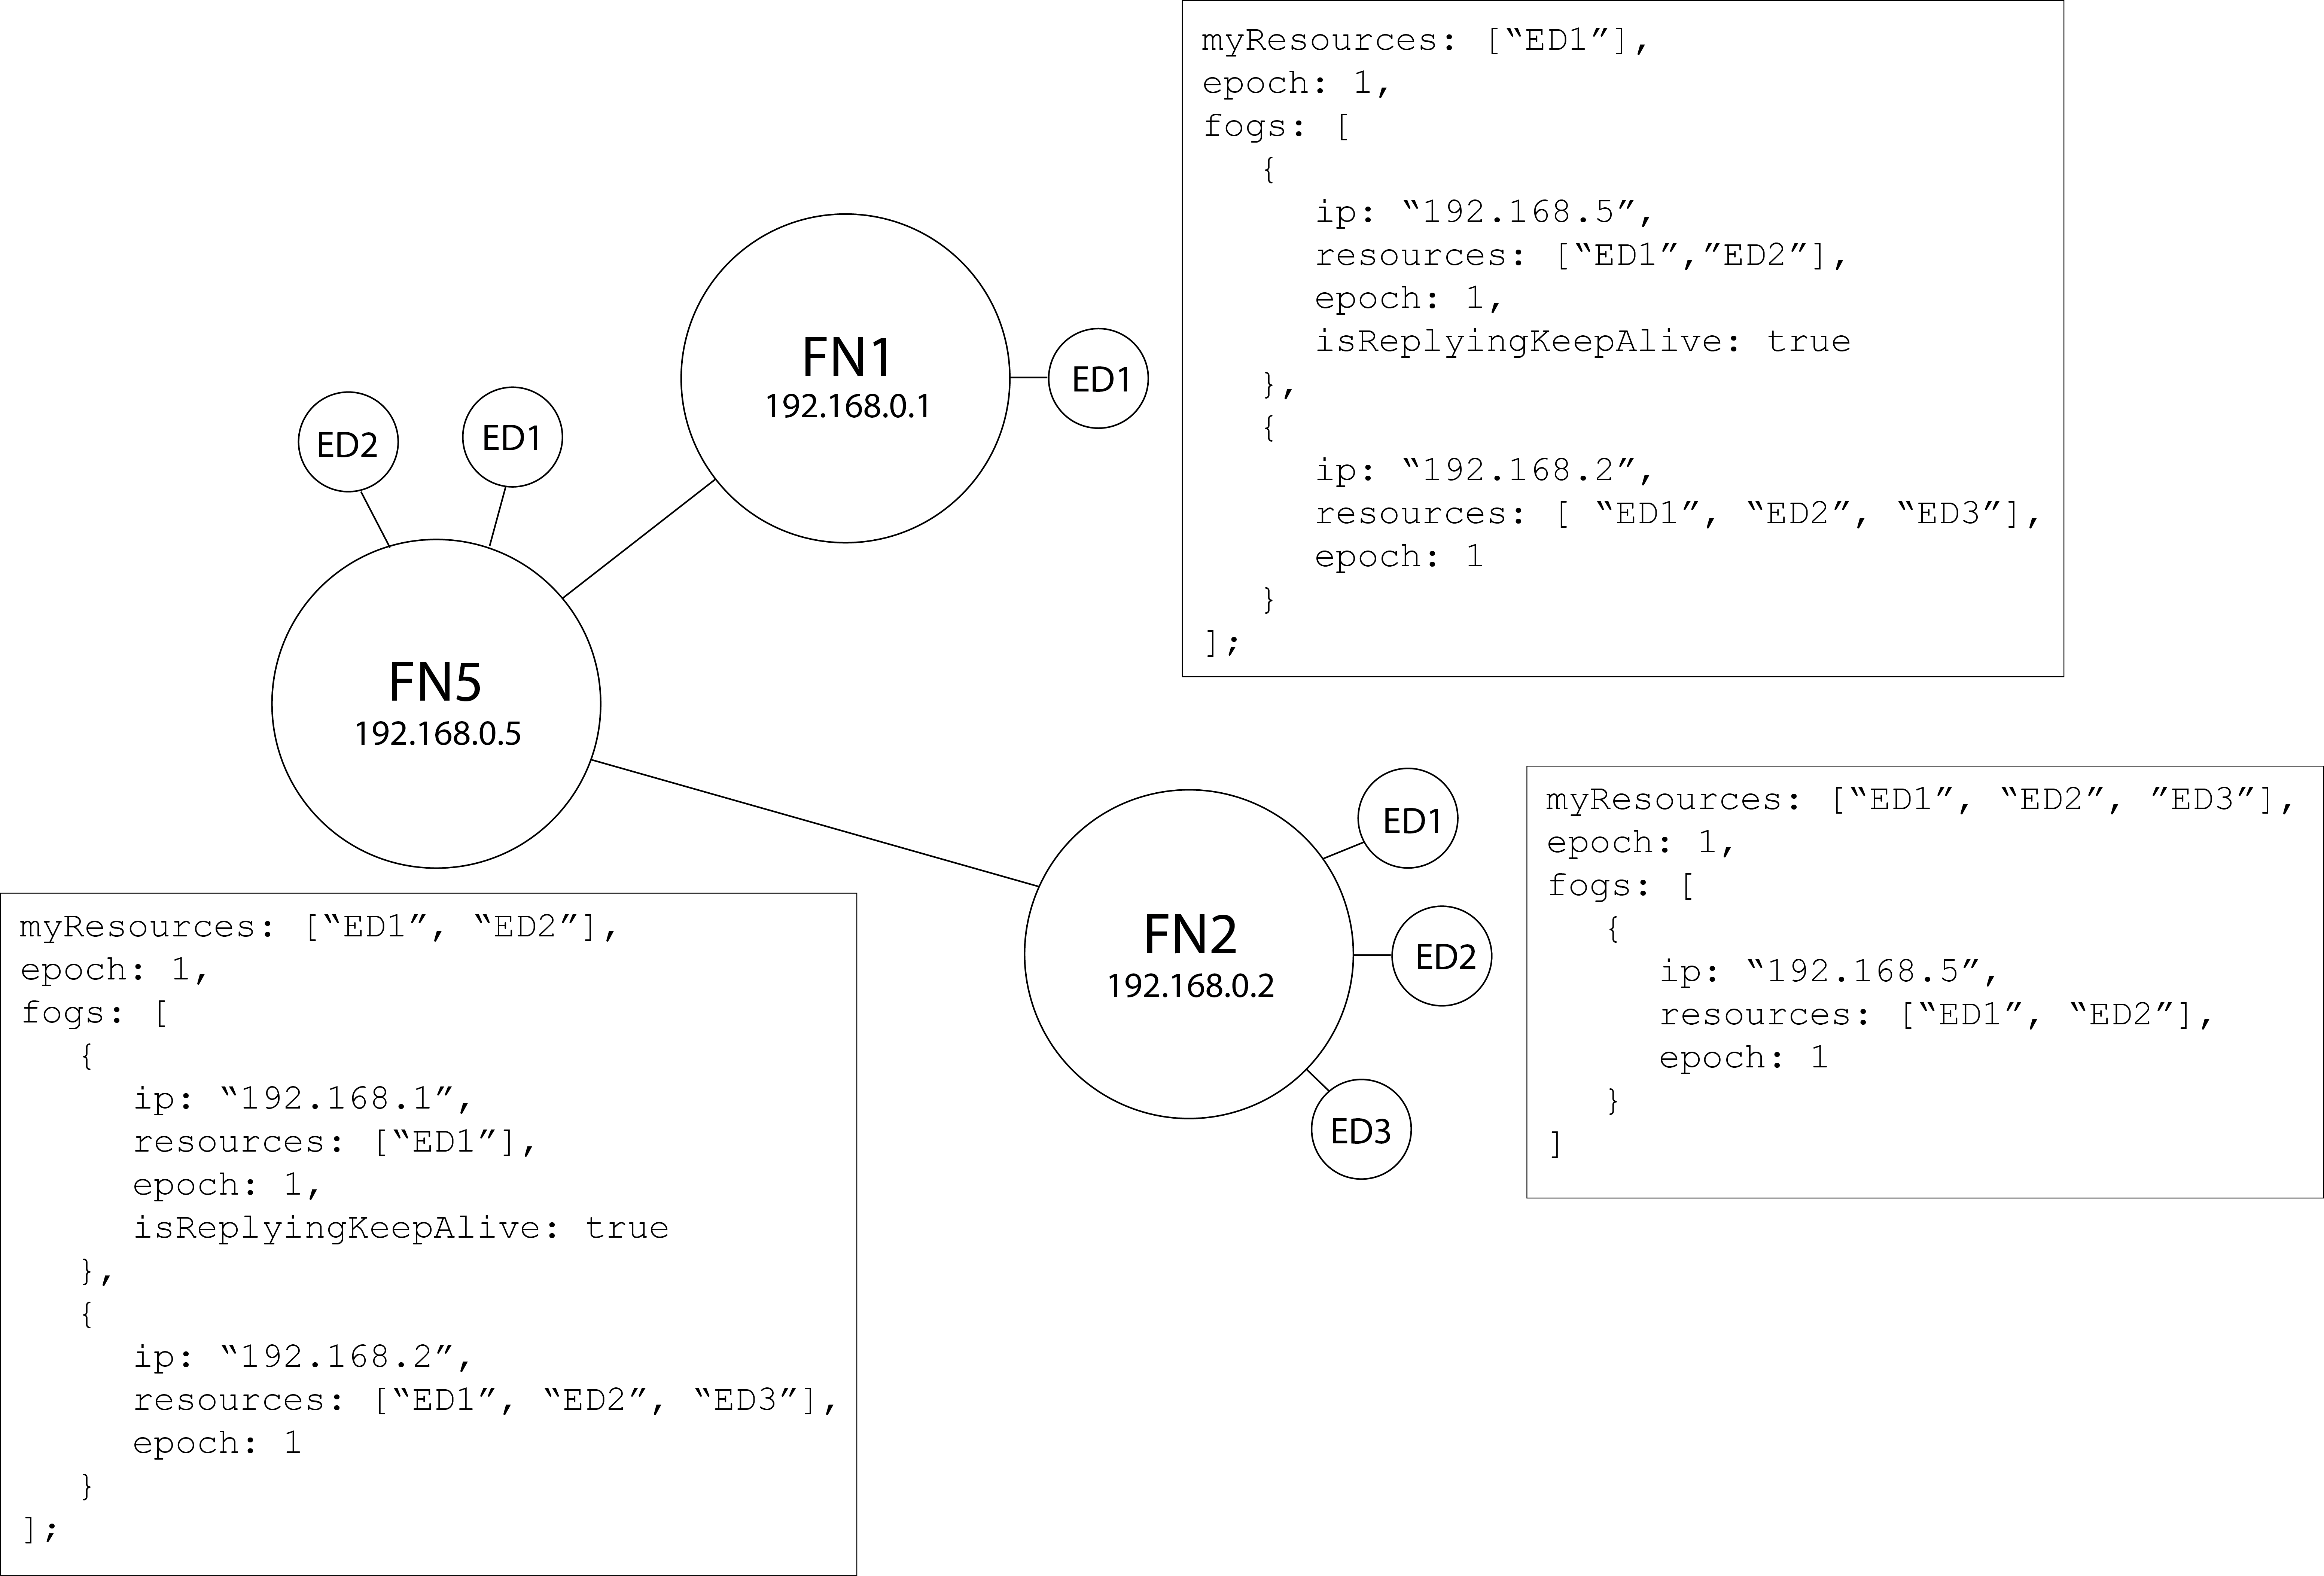
\includegraphics[width=.8\textwidth]{fig9.png}
    \caption%[This figure has a shorter caption now]%
    {\label{fig:fig9} Nodo removido da lista de recursos.}
\end{figure}

O terceiro item dos cenários de teste trata de quando o nodo está normalmente em operação, porém, um de seus recursos foi alterado, seja por incremendo de um novo edge device ou
pela remoção de um.

\begin{figure}[H]
    \centering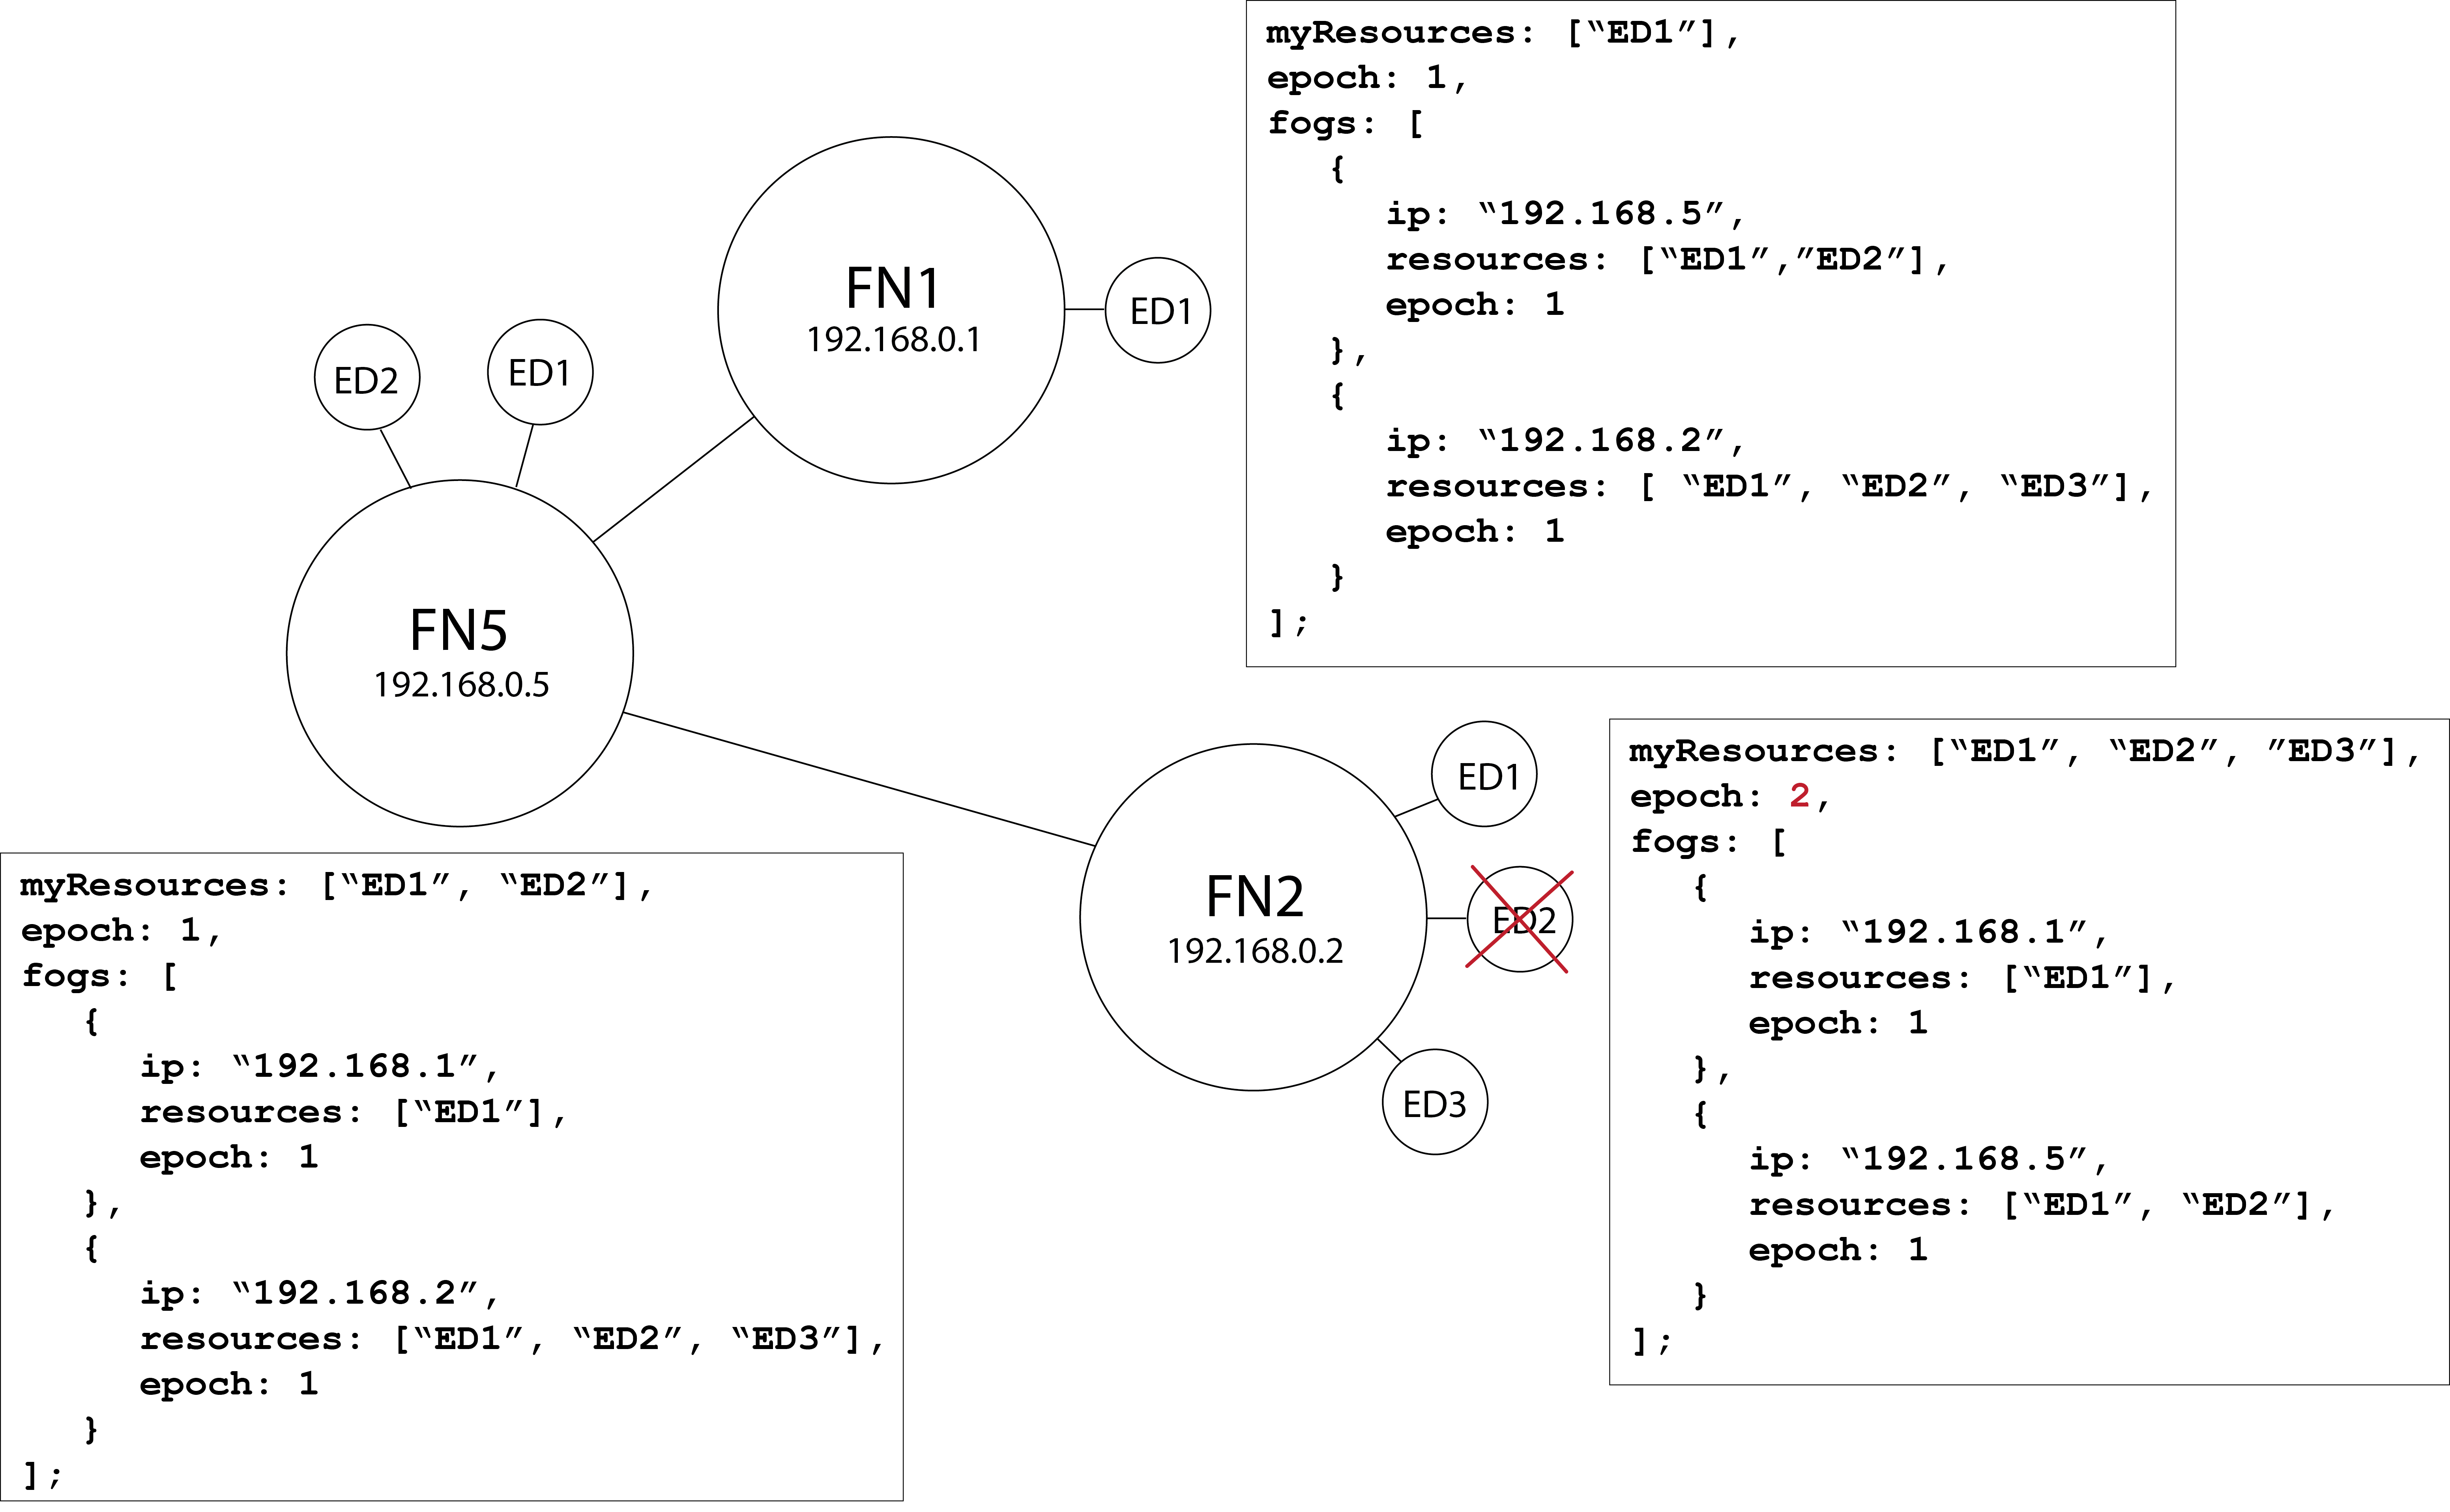
\includegraphics[width=.8\textwidth]{fig10.png} 
    \caption%[This figure has a shorter caption now]%
    {\label{fig:fig10} Edge device fora de operação.}
\end{figure}

Utilizaremos a Figura \ref{fig:fig10} como exemplo básico, e nela podemos observar que o edge device denominada ED2 vinculado ao nodo FN2 parou de funcionar.
Para este cenário, o nodo que hospeda ED2 deve estar ciente que este edge device está inoperante, e assim atualizar a sua \textit{época}.
O nodo que possui o edge device inoperante, então, terá sua época enviada juntamente com as mensagens de keep alive.
Assim, quando o nodo receber esta mensagem poderá comparar a época armazenada em sua lista de fogs com a época recebida pelo keep alive, e após a validação da divergencia realizará
um Requisição diretamente ao nodo para que possa atualizar sua lista de recursos globais.

\begin{figure}[H]
    \centering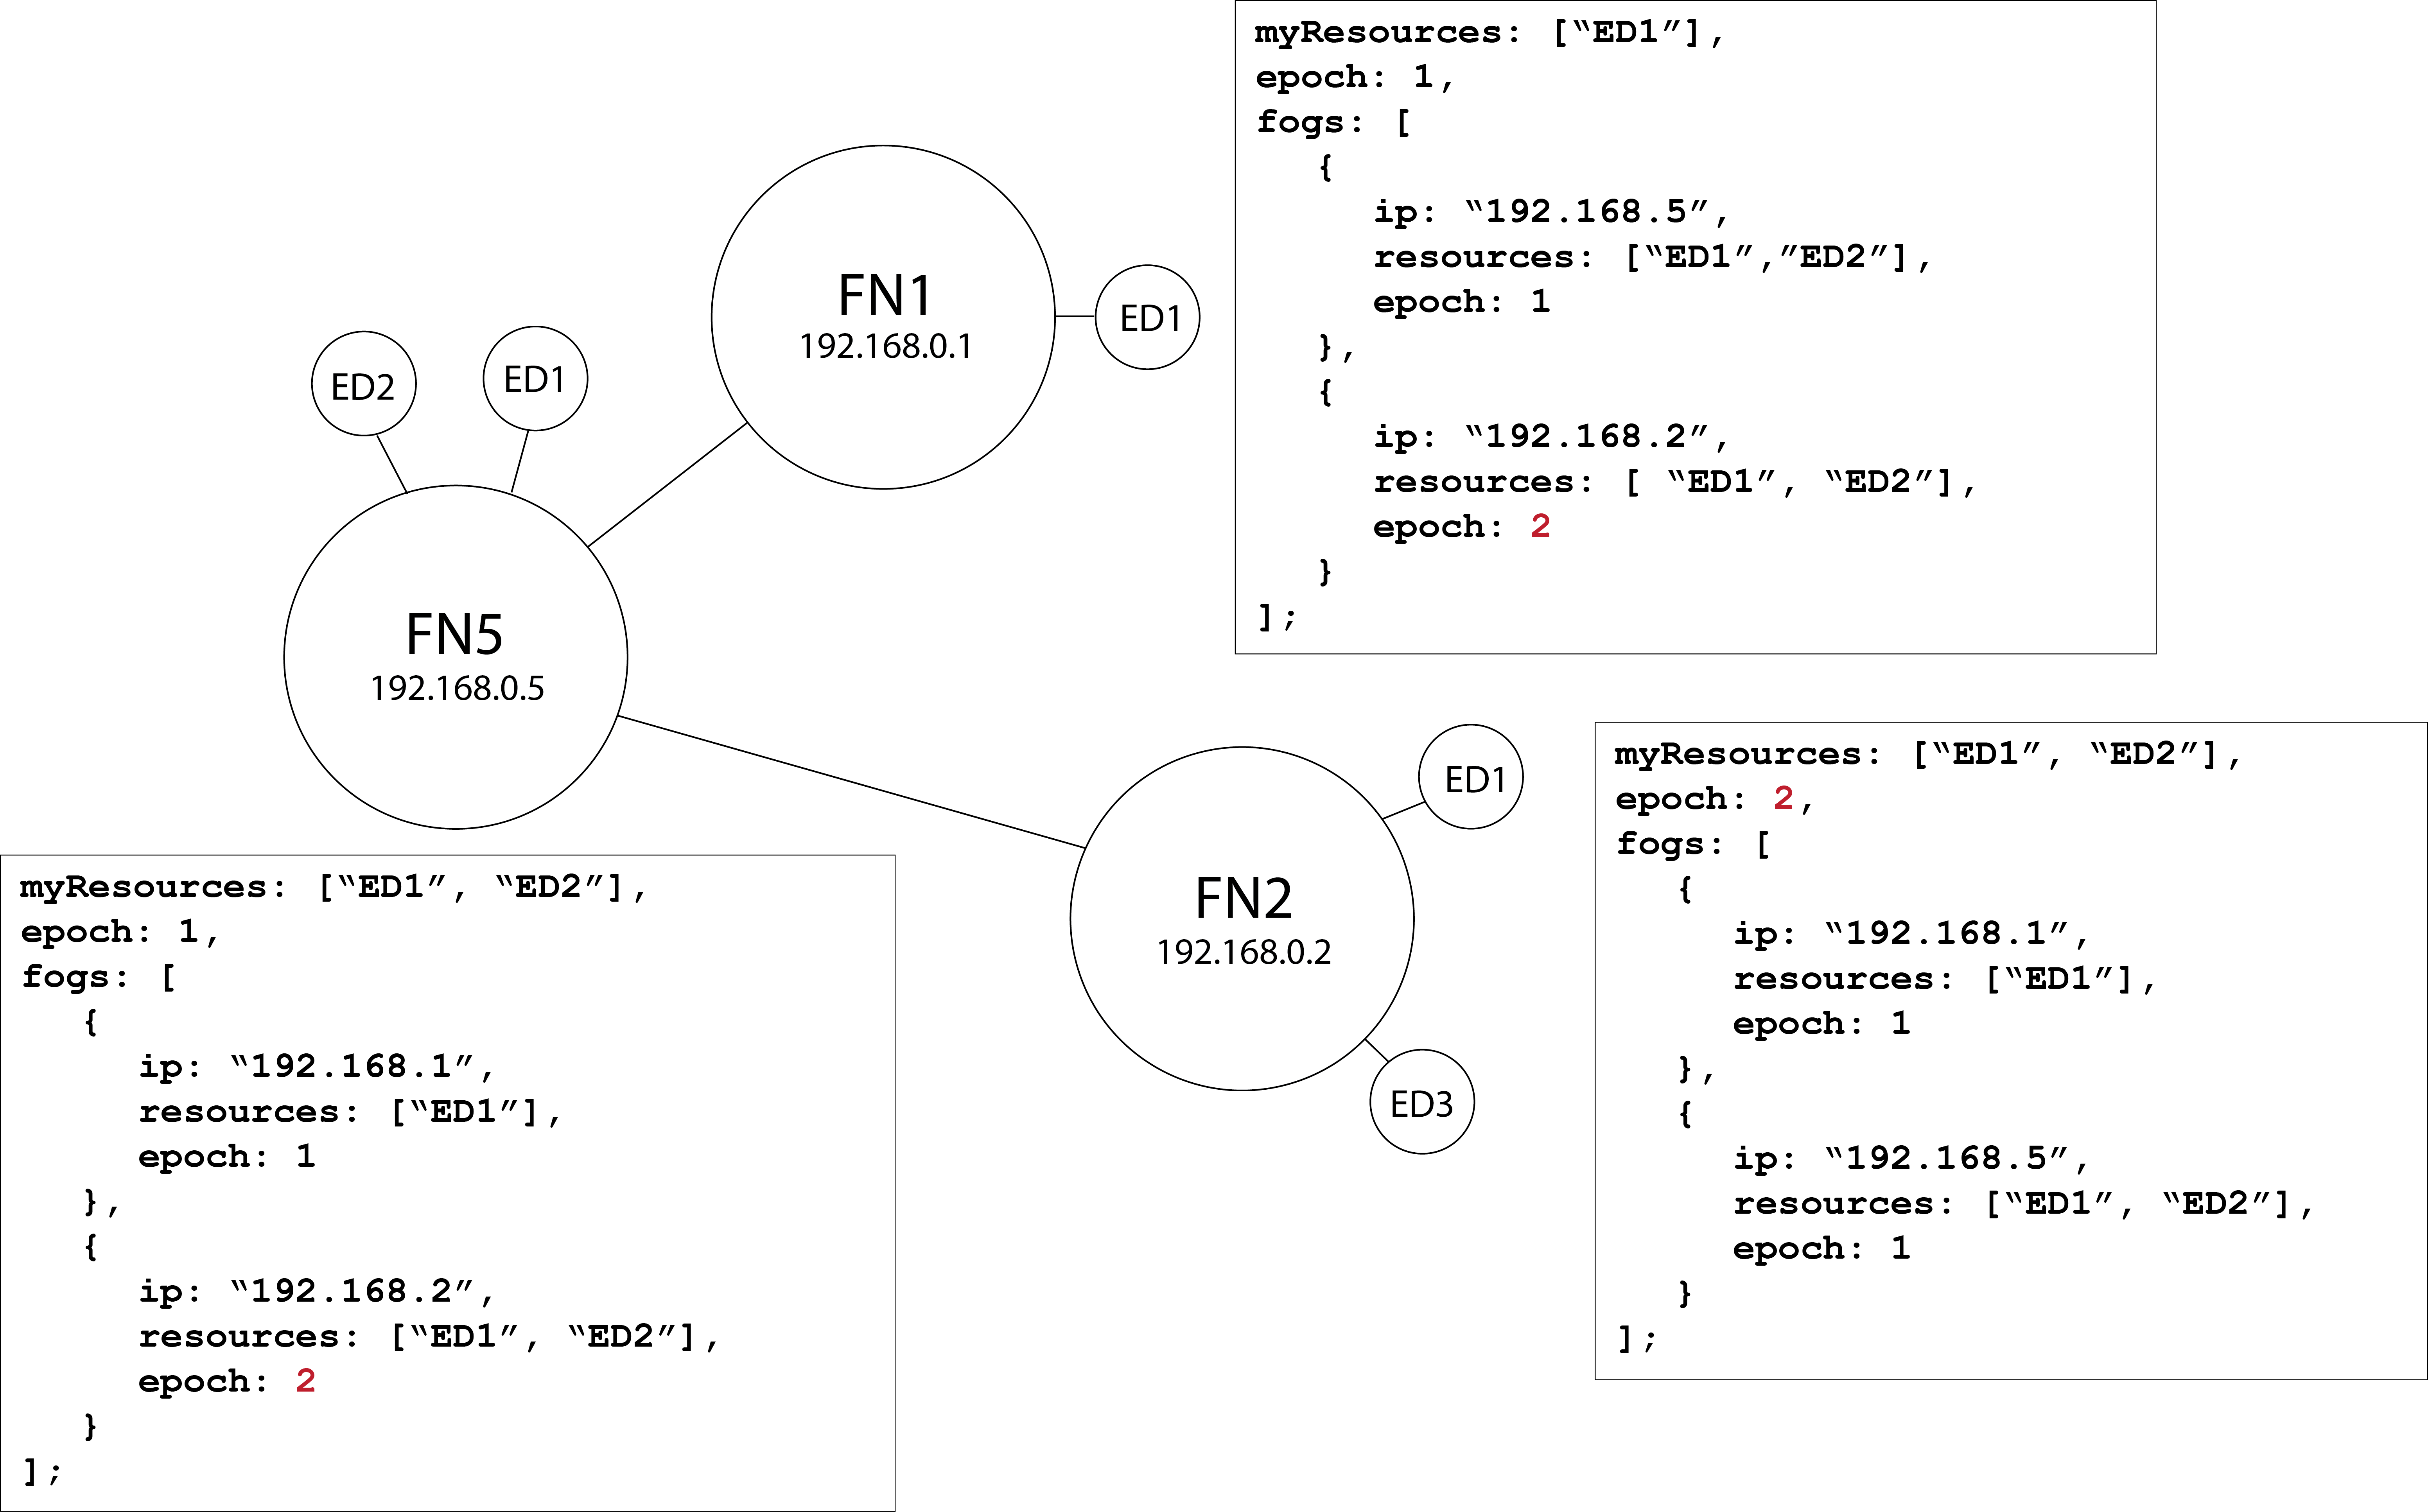
\includegraphics[width=.8\textwidth]{fig11.png} 
    \caption%[This figure has a shorter caption now]%
    {\label{fig:fig11} Estado da névoa após atualização de recursos.}
\end{figure}





\section{Estudos de caso}
% Seção: "Estudos de caso" (pelo menos 2) - pensar em alguma aplicação, onde por exemplo tens um conjunto amplo de recursos (por exemplo, diversos sensores e atuadores, luminárias, cameras, etc, tipo o prédio 32 da PUC). Pensa que os usuários de tal ambiente (alunos, professores, etc) são potenciais fornecedores de recursos (o alunos é identificado por seu smartphone na rede local e está inscrito em diversas disciplinas). Informações sobre presença (ou ausência) poderiam ser registradas, o aluno poderia ser informado sobre a sala/lab que deveria se dirigir juntamente com o tópico da aula... Sei lá! Tem que pensar em uma forma se simular, de maneira simplificada, um cenário como esse.
